\documentclass[12pt, a4paper]{article}
\usepackage{gset}
\usepackage{preamble}
\graphicspath{ {./} }
\begin{document}
	\maintitle{Дискретная математика. Домашнее задание 3}
	\textbf{Д3.1}. Функции из A в B — это по определению подмножества A × B и потому к ним применимы
	теоретико-множественные операции. Пусть f, g — две функции из A в B. Верно ли, что всегда а) их
	объединение — тоже функция; б) их пересечение — тоже функция?
	\bspace
	1) Для функции верно, что каждому аргументу соответствует одно значение. При объединении 2 функций может получиться так, что одному аргументу будут соответствовать 2 значения. Так, например, если взять функции $f(x) = x^2$, $g(x) = x + 1$. Аргументу 2 в полученном объединении будут соответствовать пары (2, 3) и (2, 4). Таким образом объединие двух функций не всегда является функцией.\\
	\\
	2) Ответ: да. Докажем, используя закон контрапозиции. Пусть $f(x) \cap g(x)$ не функция. Тогда должно выпольняться условие, что существует такой $x \in A$, которому в множестве пересечения функция соответствует больше одной пары. Пусть это верно, тогда обе эти пары есть как в множестве $f(x)$, так и в $g(x)$. Тогда $f(x)$ и $g(x)$ не функции. Таким образом, по закону контрапозии, пересечение функций является функцией.
	\bspace
	\textbf{Д3.2}. Докажите, что функция $f: (x_0, x_1, \cdots, x_{n - 1}) \lif (x_0 + 0, x_1 + 1, \cdots, x_{n - 1} + n - 1)$ является биекцией
	из множества неубывающих целочисленных последовательностей длины n в множество строго возраcтающих целочисленных последовательностей длины n. В неубывающей последовательности каждый
	член не меньше предыдущего, в строго возрастающей каждый член больше предыдущего.
	\bspace
	Докажем, что f - инъекция. Докажем от противного. Если f(x) не сюрьекция, то существуют две неубывающих последовательности A и B, такие что $f(A) = f(B) = C$. Поэлементно сравним $f(A)$ и $f(B)$. \\
	$c_0 = a_0 + 0 = b_0 + 0  \lif a_0 = b_0 \\
	c_1 = a_1 + 1 = b_1 + 1 \lif a_1 = b_1 \\
	\vdots \\
	c_{n - 1} = a_{n - 1} + n - 1 = b_{n - 1} + n - 1 \lif a_{n - 1} = b_{n - 1}$. Получаем, что A = B. Значит, не существует таких неубывающих последовательностей A и B, таких, что $f(A) = f(B) = C$. Таким образом f(x) - инъекция. \\
	Докажем, что f(x) - сюрьекция. Покажем, как восстановить по произвольной возрастающей целочисленную последовательности Y такую неубывающую целочисленную последовательность X, чтобы $f(X) = Y$.
	Необходимо, чтобы $(x_0 + 0 = y_0) \land (x_1 + 1 = y_1) \land \cdots \land (x_{n - 1} + n - 1 = y_{n - 1})$. Таким образом $X = (y_0 - 0, y_1 - 1, \cdots, y_{n - 1} - n + 1)$. Докажем, что полученная последовательность Х является неубывающей: Из того, что Y - возрастающая целочисленная последовательность следует, что $\forall i, j : j \geq i | y_i + (j - i) \leq y_j$, значит верно $j \geq i | y_i - i \leq y_i + (j - i) - j $. Значит Х - неубывающая последовательность. Таким образом, f(x) - сюрьекция.\\
	Так как f(x) инъекция и сюрьекция, то f(x) - биекция.
	\bspace
	\textbf{Д3.3} Функция f из множества [10] = \{0, 1, 2, 3, 4, 5, 6, 7, 8, 9\} в [10] сопоставляет x последнюю цифру
	десятичной записи $x^2 + 1$. Последовательность функций $f_n$ определена как $f_0 = f, f_{n+1} = f$ ◦ $f_n$. \\
	Докажите, что $f_{2023}(3)$ $\neq$ $f_{2023}(4)$.\\
	Для каждого числа из [10] посчитаем f(x). \\
	$\{f(0), f(1), f(2) \cdots, f(9)\} = \{1, 2, 5, 0, 7, 6, 7, 0, 5, 2\}$.\bspace
	\[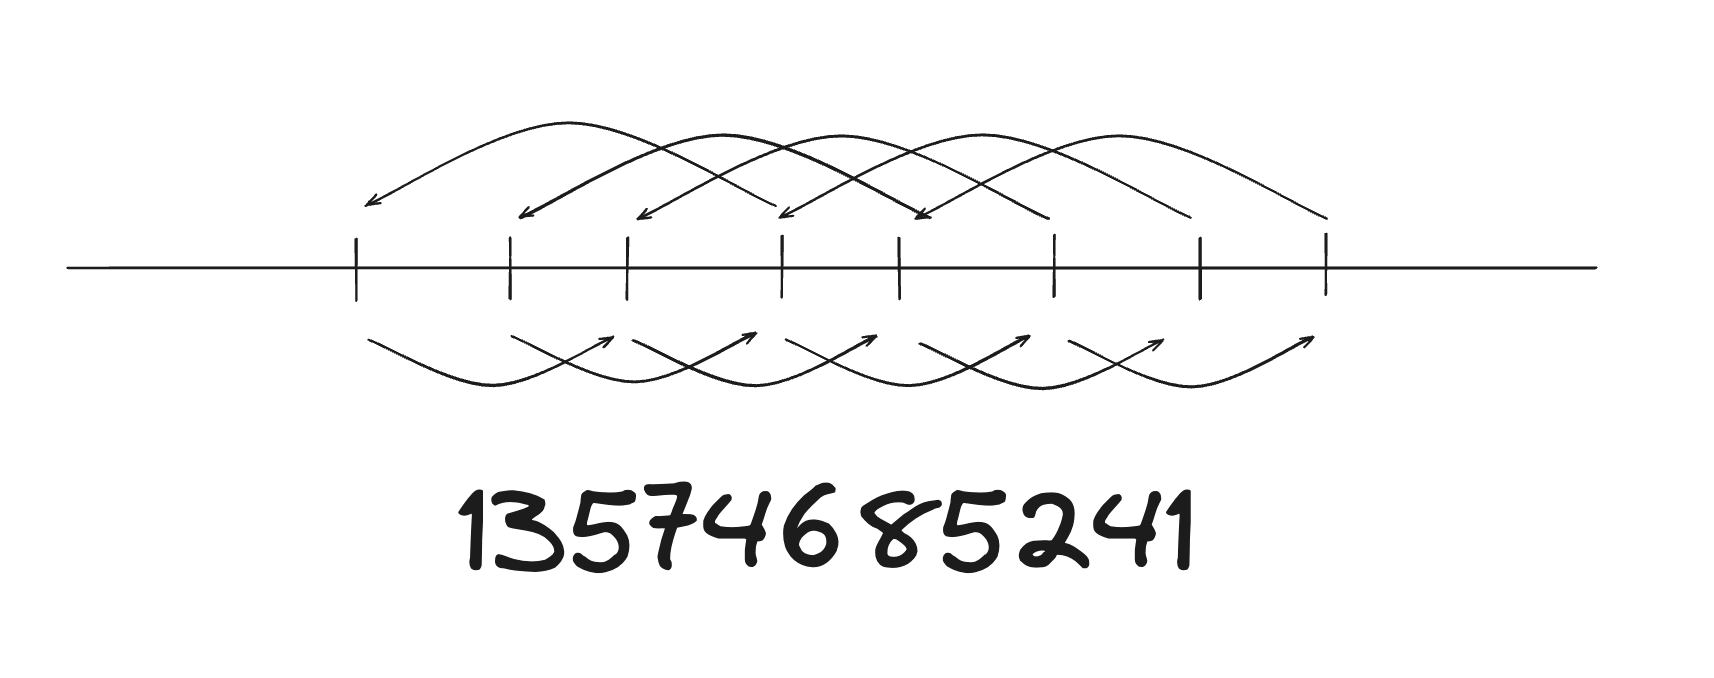
\includegraphics[width=125mm]{img}\]
	\bspace
	На картинке я показал нагляднее, как происходят переходы из одного состояния в другое, после применения функции f(x). Таким образом $f_{2023}(3) = f_{2022}(0)$, $f_{2023}(4) = f_{2021}(0)$. Так как в графе нет петель или $\forall x \in [10]: f(x) \neq x$, то $(f $ ◦ $f_{2021})(0) \neq f_{2021}(0)$, значит и  $f_{2023}(3)$ $\neq$ $f_{2023}(4)$
	\bspace
	\textbf{Д3.4}
	Пусть $f : A \lif B, g : B \lif A$ — две функции, причём g ◦ f — тождественная функция на A (то есть
	для любого $x \in A$ выполнено (g ◦ f)(x) = x). Докажите, что g — сюръекция, а f — инъекция.
	\bspace
	Докажем, что $f$ - инъекция. Докажем от противного. Если $f$ не инъекция, то $\exists (x, y): x \neq y | f(x) = f(y) = C$. Тогда так как $g$ ◦ $f$ тождественная функция, то $(g(C) = x) \land (g(C) = y)$. Значит $x = y$. Противоречие. Значит $f$ - инъекция. \\
	Докажем, что $g$ - сюръекция. По определению функции $Range(f) \subseteq B$. Так как $f$ - инъекция, значит для каждого $x \in A$ сущестует $g(f(x)) = x$. Значит g - сюрьекция.
	\end{document}